---
id: tkz-euclide-ejemplo-60
title: "Octágono regular"
description: "Creación de un octágono regular"
keywords: [poligono, octagono, taller3]
tags: [tkzDefRegPolygon,tkzDrawPolygon]
sort: 60
---
\documentclass[tikz,border=2mm]{standalone}
\usepackage{xcolor}
\usepackage{tkz-base}
\usepackage{tkz-euclide}

\begin{document}
    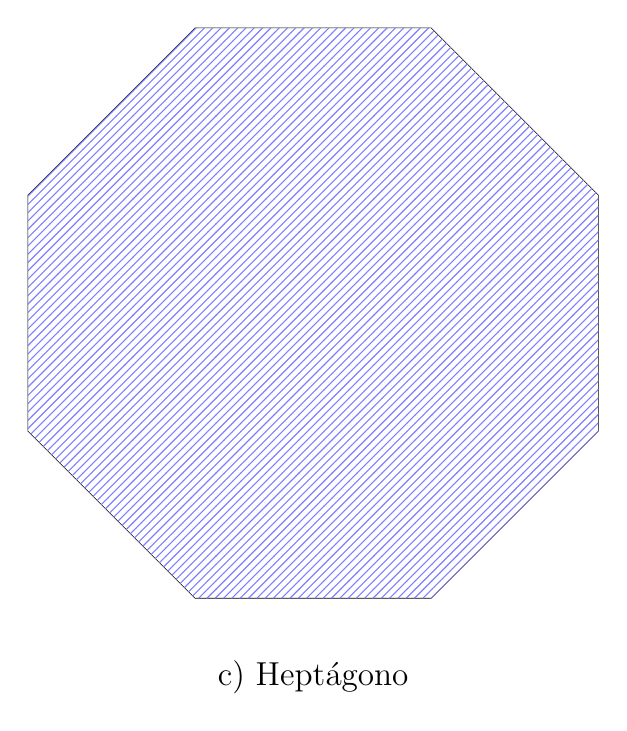
\begin{tikzpicture}
        % Paso 1: Define un punto central y uno del perímetro
        \tkzDefPoint(20,1){C} % centro
        \tkzDefPoint(23,1){D} % vértice perimetral   

        % Paso 2: Define polígono regular de 8 lados
        % con centro C y punto perimetral D
        % con vêrtices llamaodos R1,R2,...,R8.
        \tkzDefRegPolygon[side,sides=8,name=R](C,D)

        % Paso 3: Dibuja el octágono
        \tkzDrawPolygon(R1,R...,R8)

        % Paso 4: Rellena polígono con un patrón de líneas zules
        \tkzFillPolygon[pattern=north east lines,pattern color=blue!50](R1,R...,R8)
        
        % Paso 5: Coloca una leyenda debajo de la figura
        \tkzText(21.5,0){\large{c) Heptágono}}        
    \end{tikzpicture}
\end{document}